\documentclass[12pt]{article}

\usepackage{wrapfig}
\usepackage{../HBSuerDemir}

\begin{document}


	\hPage{b1p2/286}

	\begin{large} %title
	\textsc{C. Rotation of Coordinate axes and Application:} \\
	\end{large}

A transformation which rotates (turns) all points of a figure through the same angle $\Theta$ about a given point O is called a \textit{rotation}.

The point O is the \textit{center of rotation} and $\Theta$ the \textit{angle of rotation.} $\Theta$ is considered positive (negative) when measured counterclockwise (clockwise).

	\begin{wrapfigure}{r}{0.5\textwidth} %figure
	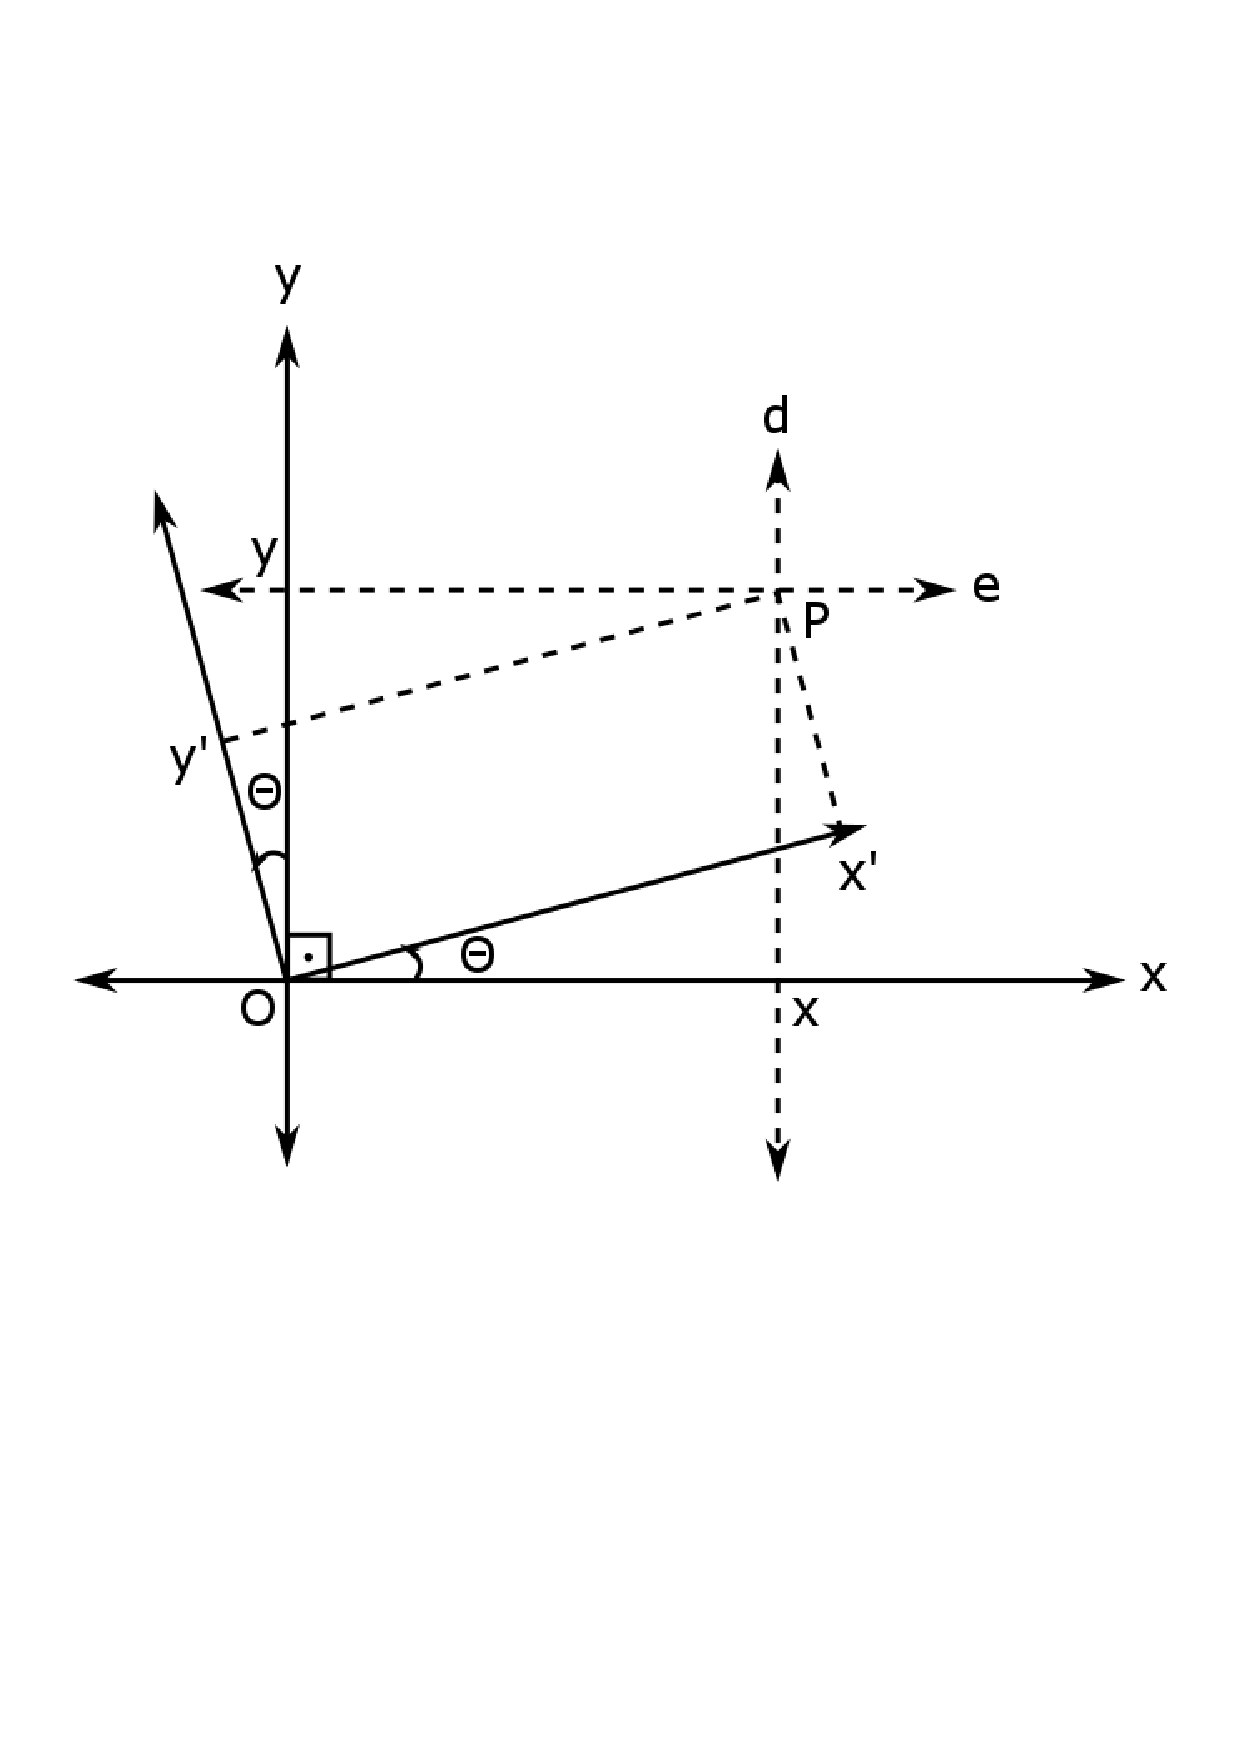
\includegraphics [trim={0 10cm 0 4cm},clip, width=0.5\textwidth]{images/b1p2-286-fig01.pdf}
	\end{wrapfigure}

A rotation with center at the origin and with angle $\Theta$ rotates the coordinate system Oxy into a new coordinate system Ox$^\prime$y$^\prime$.

To obtain the transforming formulas for coordinates x, y and x$^\prime$, y$^\prime$ of the same point P in the systems Oxy and Ox$^\prime$y$^\prime$, consider the lines d and e through P and perpendicular to Ox and Oy respectively.

The normal equations of d and e in Oxy system are

	\begin{align*} %equation cases
		&\begin{cases} 
		d: x^\prime \cos (- \Theta )  + y^\prime \sin (- \Theta ) - x = 0 \\
		e: x^\prime \cos (\frac{\pi}{2} - \Theta ) + y^\prime \sin (\frac{\pi}{2} - \Theta ) - y = 0
		\end{cases}
			\noindent \\ \textnormal{or} \\
		&\begin{cases} 
		x^\prime \cos \Theta - y^\prime \sin \Theta - x = 0  \\
		x^\prime \sin \Theta + y^\prime \cos \Theta -y = 0 \\
		\end{cases}
	\end{align*}

\noindent from which we have the transforming formulas:

	\begin{align*} %equations
	\underline{\textrm{From new to old}}&  & \underline{\textrm{From old to new}} &\\
	x = x' \cos\Theta - y' \sin\Theta  &  & x' = x \cos\Theta + y \sin\Theta& \\
	y = x' \sin\Theta + y' \cos\Theta &  & y'= -x \sin\Theta + \cos\Theta&
	\end{align*}

\underline{Application to SDE}: \\

Let $\operatorname*{f}(x,y) = 0$ be an equation. Then $\operatorname*{f}(x'\cos\Theta-y'\sin\Theta$


\end{document}